7. \begin{figure}[ht!]
\center{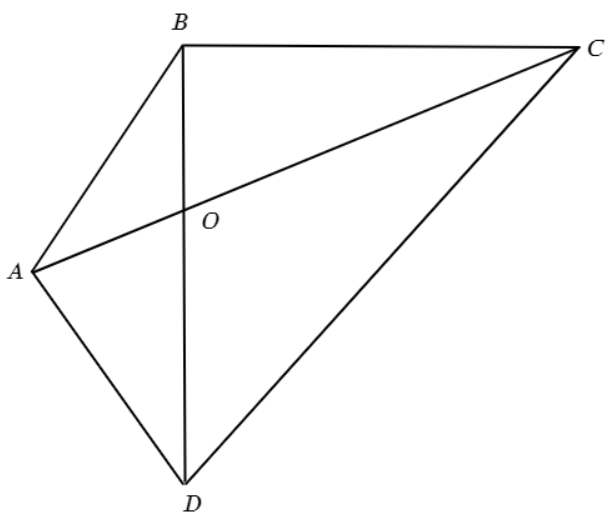
\includegraphics[scale=0.35]{g7.png}}
\end{figure}\\
Запишем четыре неравенства треугольника: $AO+OD>AD,\ BO+AO>AB,\ BO+OC>BC,\ OC+OD>CD.$ После сложения этих неравенств получим $2AO+2OC+2BO+2OD>AB+BC+CD+AD,\ 2(AC+BD)>P,\ AC+BD>\cfrac{P}{2},$ ч.т.д.\\
